\documentclass{article}
\usepackage[final]{nips_2017}
\usepackage[utf8]{inputenc} % allow utf-8 input
\usepackage[T1]{fontenc}    % use 8-bit T1 fonts
\usepackage{hyperref}       % hyperlinks
\usepackage{url}            % simple URL typesetting
\usepackage{booktabs}       % professional-quality tables
\usepackage{amsfonts}       % blackboard math symbols
\usepackage{nicefrac}       % compact symbols for 1/2, etc.
\usepackage{microtype}      % microtypography
\usepackage{graphicx}
\usepackage[font=small, labelfont=bf]{caption}
\usepackage{subcaption}
\usepackage{float}
\usepackage{amsmath}
\title{Graph-Based Classification of Rock Climbing Difficulties}

\author{
  Rafael Hinojosa \\
  Microsoft Corporation \\
  Stanford University \\
  \texttt{rahinojo@stanford.edu} \\ 
  \And
  Cheng-Hao Tai \\
  Microsoft Corporation \\
  Stanford University \\
  \texttt{c2tai@stanford.edu} \\
  \And
  Aaron Wu \\
  Evisort Inc. \\
  - \\
  \texttt{aaron@evisort.com} \\
}

\begin{document}

\begin{center}

\includegraphics[width=3cm, height=0.7cm]{CS230}
\end{center}

\maketitle

\section{Introduction}	
Given the recent increase in rock climbing's popularity, we want to create a neural network for classifying a given climbing route (a.k.a. problem) into a suitable difficulty category. This tool could either speed up or replace traditionally heuristic-based approachs to ranking climbing problems, thereby lowering the barrier of entry for anyone seeking to create their own routes. We plan to solve this problem using a classifier built for the "Moonboard" apparatus --- a modular climbing wall of fixed dimensions and pre-set hold configurations (Figure 1). 

\section{Dataset}
On their \href{https://moonboard.com/}{website}, Moonboard hosts a database of Moonboard climbing routes (see example in Figure 1b) that have been created and ranked by the global climbing community. For a given hold configuration (i.e. Moonboard 2016), routes are denoted using multi-colored circles superimposed on a stock Moonboard image. These circles specify a hold set and define a problem. Our proposed schema is:

\begin{itemize}
\setlength\itemsep{0.1em}
\item \texttt{Problem ID : int}
\item \texttt{Difficulty : int}
\item \texttt{Rating : int}
\item \texttt{Comments : string}
\item \texttt{Holds : list of tuples}
\end{itemize}

\begin{figure}
\centering
\begin{subfigure}{.48\textwidth}
  \centering
  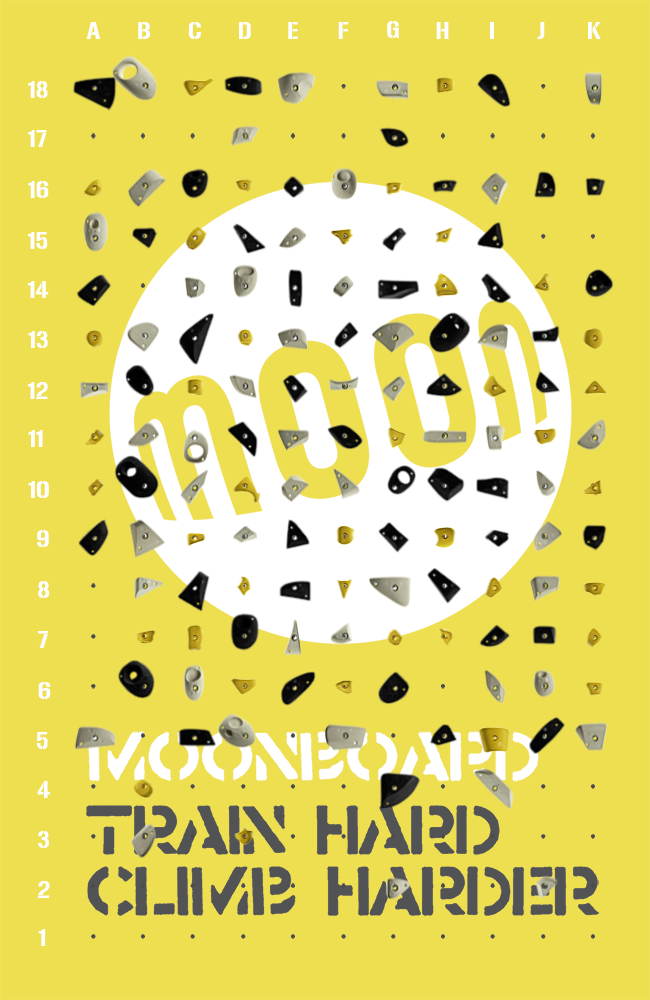
\includegraphics[width=.8\linewidth]{moonboard_stock}
  \caption{Stock Moonboard 2016 configuration}
  \label{fig: Stock Moonboard}
\end{subfigure}
\begin{subfigure}{.48\textwidth}
  \centering
  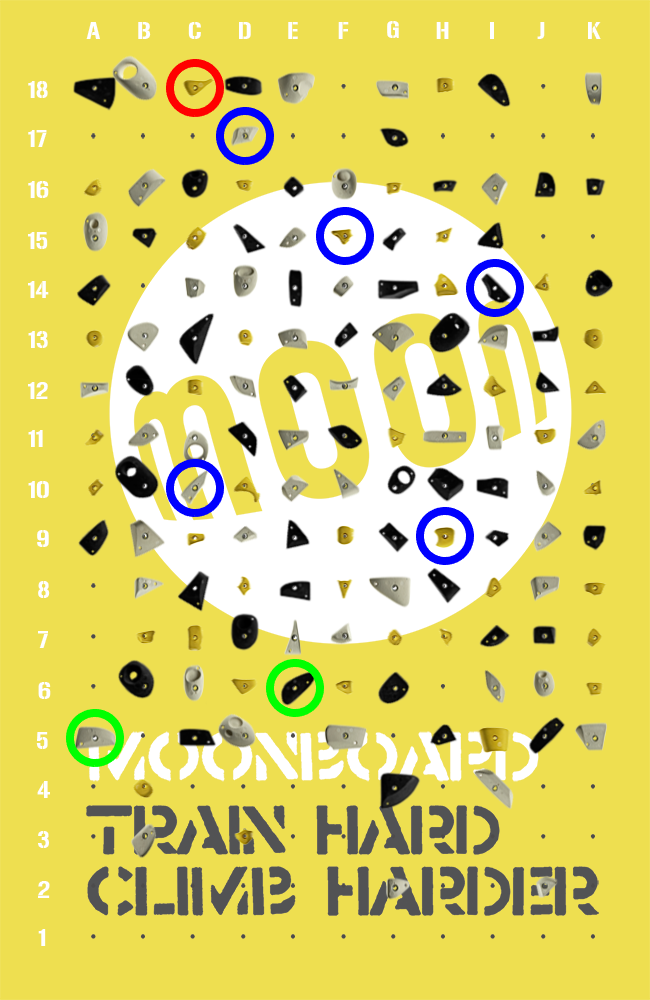
\includegraphics[width=.8\linewidth]{moonboard_1}
  \caption{A specific Moonboard problem}
  \label{fig: Moonboard Problem}
\end{subfigure}
\caption{Moonboard training apparatus showing a specific Moonboard problem}
\end{figure}

\begin{figure}
\centering
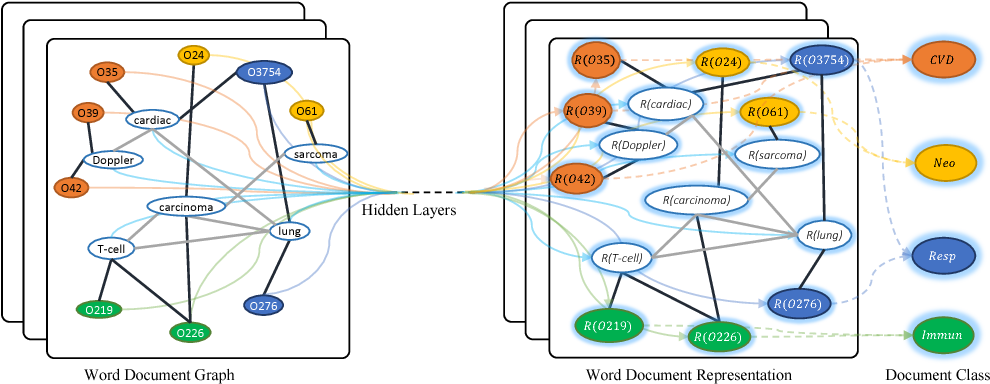
\includegraphics[width=.8\linewidth]{textGCN}
\caption{A heterogenous corpus graph for document classification using a Text Graph Convolutional Network [3]. Nodes come in 2 types: document entities and word entities. The different colors correspond to different node categories (notice only document nodes are colored). A direct analogy to Moonboard problems can be made by substituting documents for problems and holds for nodes.}
\label{fig: Corpus graph for Text Graph Convolutional Network}
\end{figure}

\section{Preprocessing and Learning Method}
We plan to mine this data from the Moonboard webpage and structure it into a graph upon which we will apply ideas from [3] which solves text classification tasks using a Text Graph Convolutional Network (GCN) (Figure 2). While the authors of [3] organized their heterogeneous corpus graph using documents and words as nodes with global co-occurrence / TFIDF scores as edge weights, we will adapt this to a Moonboard scope. In our application, document nodes are replaced by problem nodes, word nodes by hold nodes. The idea is that just as documents are composed of words, Moonboard problems are composed of holds. Tangentially, we'd also like to implement  [2] which presents a simplified version of the Text GCN that actually performed better on the same text classification task as [3]. Our proposed loss function is multi-class cross-entropy.

\section{Evaluation}
To evaluate our model, we plan to use binary classification metrics (i.e. accuracy, precision, recall, and F-score) extended to a multi-class classification use case. Since there are many distinct Moonboard difficulty ratings (around 10), we plan to perform model evaluation on each of these difficulty settings so that we're able to easily diagnose class-dependent model issues (i.e. data imbalance, overfitting one class). For the Moonboard 2016 hold configuration, there are approximately 28,000 unique problems on Moonboard's server which will correspond to a total dataset size of 28,000 samples. We plan to use a 80-20 split to create our training and test datasets and use hold-out subsets of the training set to evaluate model performance before final validation on the test set. 

\section{Additional Challenges}
Finally, if our classifier succeeds, we wish to extend our project in one of two ways: (1) a generative model [1] that can produce a new Moonboard problem, given a specific difficulty and (2) experiment with ways to overcome a significant GCN limitation (needing to retrain entire graph for every new inference sample).

\section*{References}
\medskip
\small

[1] Mirza, M. \& Osindero, S. \ Conditional Generative Adversarial Nets \ {\it arXiv:1411.1784} \ (2014)

[2] Wu, F., Zhang, T., de Souza Jr., A., Fifty, C., Yu, T., \& Weinberger, K. \ Simplifying Graph Convolutional Networks \ {\it Proceedings of the 36th International Conference on Machine Learning} \ (2019)

[3] Yao, L., Mao, C. \& Luo, Y. \ Graph Convolutional Networks for Text Classification \ {\it 33rd AAAI Conference on Artificial Intelligence (AAAI-19)}, 7370-7377 \ (2018)

\end{document}